\documentclass[14pt]{extbook}
\usepackage{multicol, enumerate, enumitem, hyperref, color, soul, setspace, parskip, fancyhdr} %General Packages
\usepackage{amssymb, amsthm, amsmath, bbm, latexsym, units, mathtools} %Math Packages
\everymath{\displaystyle} %All math in Display Style
% Packages with additional options
\usepackage[headsep=0.5cm,headheight=12pt, left=1 in,right= 1 in,top= 1 in,bottom= 1 in]{geometry}
\usepackage[usenames,dvipsnames]{xcolor}
\usepackage{dashrule}  % Package to use the command below to create lines between items
\newcommand{\litem}[1]{\item#1\hspace*{-1cm}\rule{\textwidth}{0.4pt}}
\pagestyle{fancy}
\lhead{Progress Quiz 3}
\chead{}
\rhead{Version B}
\lfoot{3148-2249}
\cfoot{}
\rfoot{Spring 2021}
\begin{document}

\begin{enumerate}
\litem{
Write the equation of the graph presented below in the form $f(x)=ax^2+bx+c$, assuming  $a=1$ or $a=-1$. Then, choose the intervals that $a, b,$ and $c$ belong to.
\begin{center}
    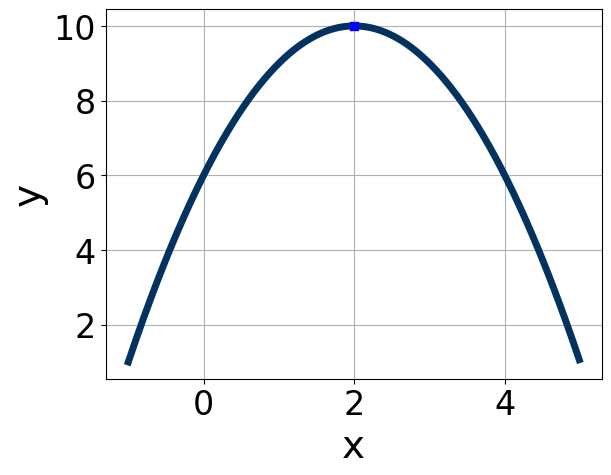
\includegraphics[width=0.5\textwidth]{../Figures/quadraticGraphToEquationCopyB.png}
\end{center}
\begin{enumerate}[label=\Alph*.]
\item \( a \in [-0.2, 1.1], \hspace*{5mm} b \in [-4, -2], \text{ and } \hspace*{5mm} c \in [12, 14] \)
\item \( a \in [-0.2, 1.1], \hspace*{5mm} b \in [4, 7], \text{ and } \hspace*{5mm} c \in [12, 14] \)
\item \( a \in [-1.5, -0.1], \hspace*{5mm} b \in [4, 7], \text{ and } \hspace*{5mm} c \in [2, 10] \)
\item \( a \in [-0.2, 1.1], \hspace*{5mm} b \in [4, 7], \text{ and } \hspace*{5mm} c \in [-6, -1] \)
\item \( a \in [-1.5, -0.1], \hspace*{5mm} b \in [-4, -2], \text{ and } \hspace*{5mm} c \in [2, 10] \)

\end{enumerate} }
\litem{
Factor the quadratic below. Then, choose the intervals that contain the constants in the form $(ax+b)(cx+d); b \leq d.$\[ 54x^{2} -57 x + 10 \]\begin{enumerate}[label=\Alph*.]
\item \( a \in [8.9, 12.9], \hspace*{5mm} b \in [-10, -1], \hspace*{5mm} c \in [2.5, 4.4], \text{ and } \hspace*{5mm} d \in [-6, 3] \)
\item \( a \in [4.3, 8.7], \hspace*{5mm} b \in [-10, -1], \hspace*{5mm} c \in [6.3, 10.6], \text{ and } \hspace*{5mm} d \in [-6, 3] \)
\item \( a \in [0.5, 1.4], \hspace*{5mm} b \in [-50, -43], \hspace*{5mm} c \in [-0.2, 1.8], \text{ and } \hspace*{5mm} d \in [-22, -7] \)
\item \( a \in [1.9, 4.1], \hspace*{5mm} b \in [-10, -1], \hspace*{5mm} c \in [25.7, 28.6], \text{ and } \hspace*{5mm} d \in [-6, 3] \)
\item \( \text{None of the above.} \)

\end{enumerate} }
\litem{
Factor the quadratic below. Then, choose the intervals that contain the constants in the form $(ax+b)(cx+d); b \leq d.$\[ 54x^{2} +21 x -20 \]\begin{enumerate}[label=\Alph*.]
\item \( a \in [7.9, 9.1], \hspace*{5mm} b \in [-5, -3], \hspace*{5mm} c \in [5.8, 6.4], \text{ and } \hspace*{5mm} d \in [-1, 7] \)
\item \( a \in [25.9, 29.9], \hspace*{5mm} b \in [-5, -3], \hspace*{5mm} c \in [1.4, 2.8], \text{ and } \hspace*{5mm} d \in [-1, 7] \)
\item \( a \in [2.7, 3.2], \hspace*{5mm} b \in [-5, -3], \hspace*{5mm} c \in [16.5, 19.6], \text{ and } \hspace*{5mm} d \in [-1, 7] \)
\item \( a \in [-1.1, 1.9], \hspace*{5mm} b \in [-32, -21], \hspace*{5mm} c \in [-0.5, 1.8], \text{ and } \hspace*{5mm} d \in [42, 52] \)
\item \( \text{None of the above.} \)

\end{enumerate} }
\litem{
Write the equation of the graph presented below in the form $f(x)=ax^2+bx+c$, assuming  $a=1$ or $a=-1$. Then, choose the intervals that $a, b,$ and $c$ belong to.
\begin{center}
    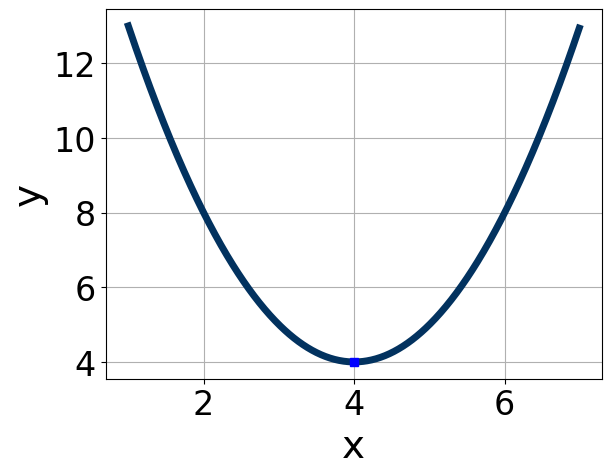
\includegraphics[width=0.5\textwidth]{../Figures/quadraticGraphToEquationB.png}
\end{center}
\begin{enumerate}[label=\Alph*.]
\item \( a \in [0, 3], \hspace*{5mm} b \in [6, 10], \text{ and } \hspace*{5mm} c \in [8, 12] \)
\item \( a \in [-5, 0], \hspace*{5mm} b \in [-8, -4], \text{ and } \hspace*{5mm} c \in [-22, -19] \)
\item \( a \in [0, 3], \hspace*{5mm} b \in [-8, -4], \text{ and } \hspace*{5mm} c \in [8, 12] \)
\item \( a \in [0, 3], \hspace*{5mm} b \in [-8, -4], \text{ and } \hspace*{5mm} c \in [18, 24] \)
\item \( a \in [-5, 0], \hspace*{5mm} b \in [6, 10], \text{ and } \hspace*{5mm} c \in [-22, -19] \)

\end{enumerate} }
\litem{
Solve the quadratic equation below. Then, choose the intervals that the solutions $x_1$ and $x_2$ belong to, with $x_1 \leq x_2$.\[ 15x^{2} +47 x + 36 = 0 \]\begin{enumerate}[label=\Alph*.]
\item \( x_1 \in [-2.11, -1.41] \text{ and } x_2 \in [-1.54, -1.24] \)
\item \( x_1 \in [-9.46, -8.66] \text{ and } x_2 \in [-0.35, 0.13] \)
\item \( x_1 \in [-27.2, -26.83] \text{ and } x_2 \in [-20.25, -19.75] \)
\item \( x_1 \in [-3, -2.37] \text{ and } x_2 \in [-1.28, -0.8] \)
\item \( x_1 \in [-5.75, -5.33] \text{ and } x_2 \in [-0.71, -0.27] \)

\end{enumerate} }
\litem{
Solve the quadratic equation below. Then, choose the intervals that the solutions belong to, with $x_1 \leq x_2$ (if they exist).\[ -11x^{2} -11 x + 7 = 0 \]\begin{enumerate}[label=\Alph*.]
\item \( x_1 \in [-1.4, 0.7] \text{ and } x_2 \in [0.9, 3.4] \)
\item \( x_1 \in [-5, -4.2] \text{ and } x_2 \in [15.4, 17] \)
\item \( x_1 \in [-2.8, -1.1] \text{ and } x_2 \in [-1.4, 0.7] \)
\item \( x_1 \in [-22, -21.1] \text{ and } x_2 \in [20.1, 21.8] \)
\item \( \text{There are no Real solutions.} \)

\end{enumerate} }
\litem{
Solve the quadratic equation below. Then, choose the intervals that the solutions belong to, with $x_1 \leq x_2$ (if they exist).\[ 18x^{2} +13 x -4 = 0 \]\begin{enumerate}[label=\Alph*.]
\item \( x_1 \in [-2.9, -0.5] \text{ and } x_2 \in [-0.43, 0.58] \)
\item \( x_1 \in [-23.6, -19.8] \text{ and } x_2 \in [20.64, 21.64] \)
\item \( x_1 \in [-17.7, -16.2] \text{ and } x_2 \in [3.45, 4.66] \)
\item \( x_1 \in [-0.7, 0] \text{ and } x_2 \in [0.74, 1.41] \)
\item \( \text{There are no Real solutions.} \)

\end{enumerate} }
\litem{
Graph the equation below.\[ f(x) = (x-1)^2 + 20 \]\begin{enumerate}[label=\Alph*.]
\begin{multicols}{2}\item 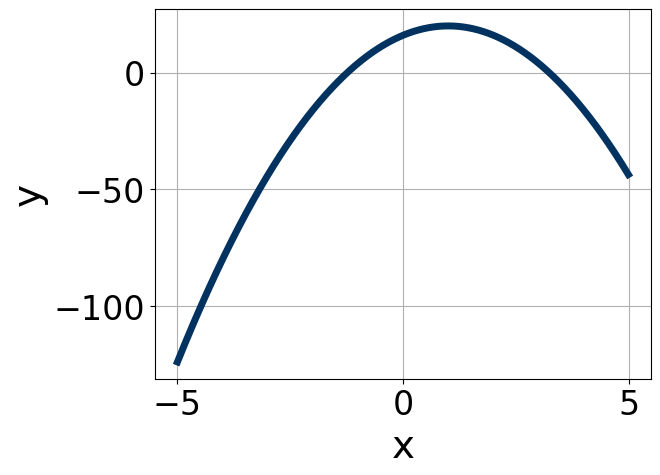
\includegraphics[width = 0.3\textwidth]{../Figures/quadraticEquationToGraphCopyAB.png}\item 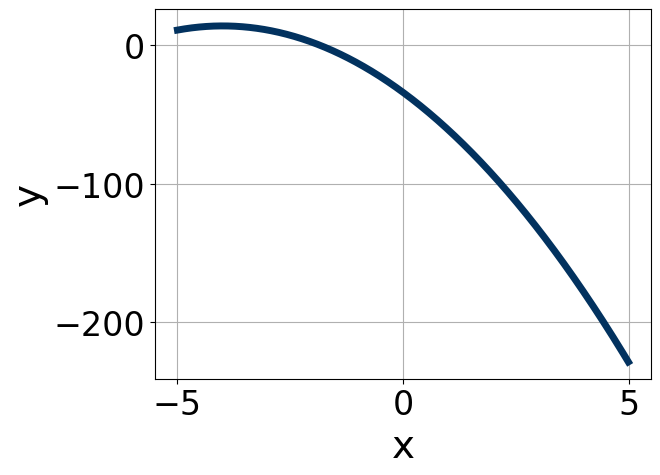
\includegraphics[width = 0.3\textwidth]{../Figures/quadraticEquationToGraphCopyBB.png}\item 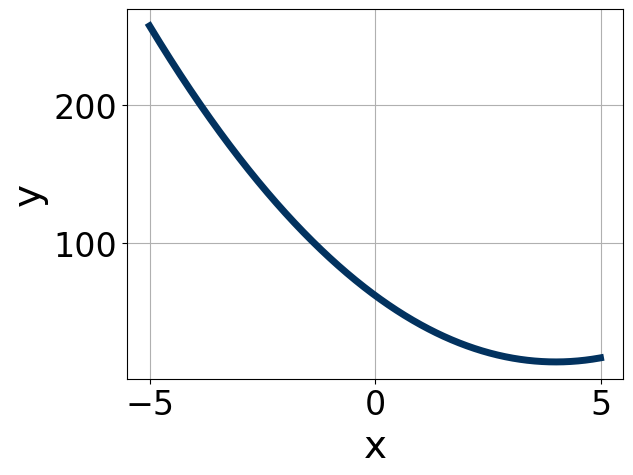
\includegraphics[width = 0.3\textwidth]{../Figures/quadraticEquationToGraphCopyCB.png}\item 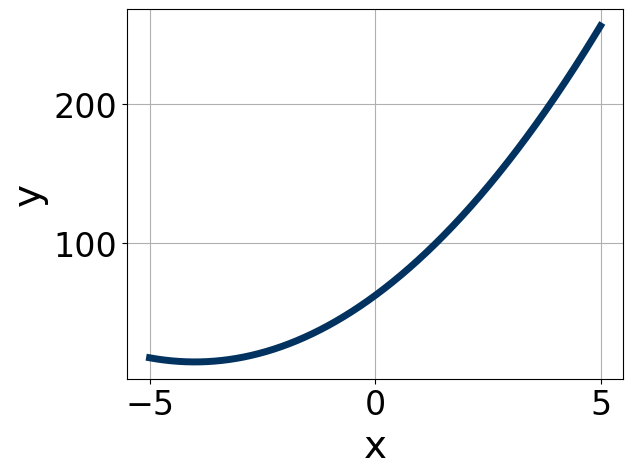
\includegraphics[width = 0.3\textwidth]{../Figures/quadraticEquationToGraphCopyDB.png}\end{multicols}\item None of the above.
\end{enumerate} }
\litem{
Graph the equation below.\[ f(x) = (x+4)^2 - 12 \]\begin{enumerate}[label=\Alph*.]
\begin{multicols}{2}\item 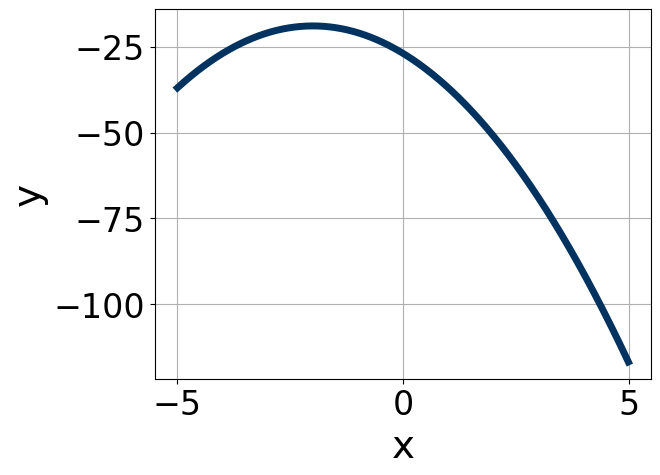
\includegraphics[width = 0.3\textwidth]{../Figures/quadraticEquationToGraphAB.png}\item 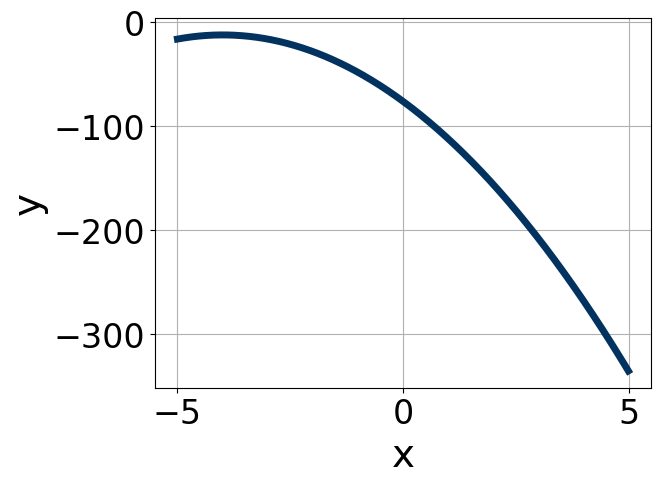
\includegraphics[width = 0.3\textwidth]{../Figures/quadraticEquationToGraphBB.png}\item 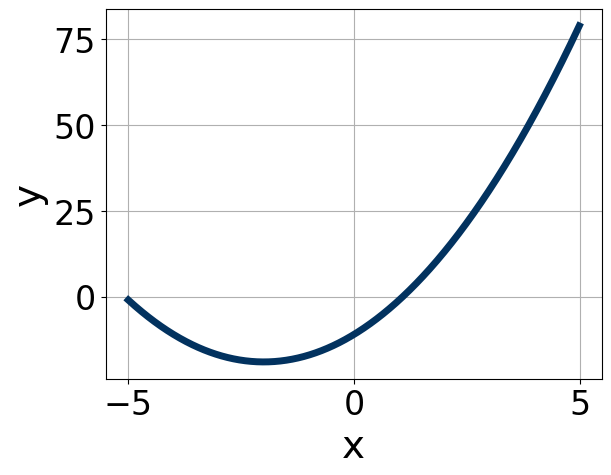
\includegraphics[width = 0.3\textwidth]{../Figures/quadraticEquationToGraphCB.png}\item 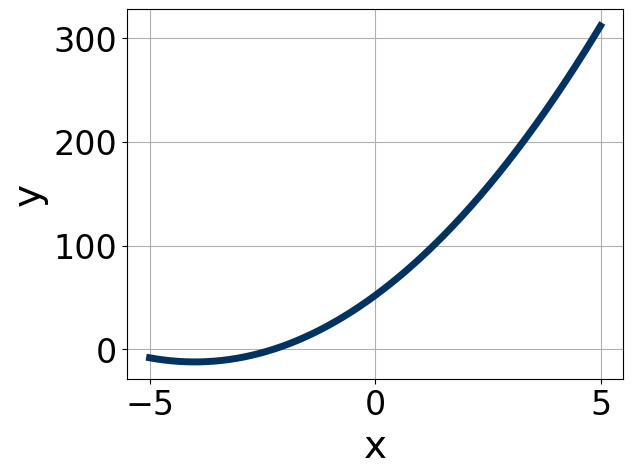
\includegraphics[width = 0.3\textwidth]{../Figures/quadraticEquationToGraphDB.png}\end{multicols}\item None of the above.
\end{enumerate} }
\litem{
Solve the quadratic equation below. Then, choose the intervals that the solutions $x_1$ and $x_2$ belong to, with $x_1 \leq x_2$.\[ 20x^{2} +69 x + 54 = 0 \]\begin{enumerate}[label=\Alph*.]
\item \( x_1 \in [-2.32, -2.22] \text{ and } x_2 \in [-1.24, -1.19] \)
\item \( x_1 \in [-6.77, -6.73] \text{ and } x_2 \in [-0.42, -0.35] \)
\item \( x_1 \in [-2.48, -2.3] \text{ and } x_2 \in [-1.14, -0.99] \)
\item \( x_1 \in [-9.1, -8.8] \text{ and } x_2 \in [-0.37, -0.24] \)
\item \( x_1 \in [-45.09, -44.99] \text{ and } x_2 \in [-24.03, -23.92] \)

\end{enumerate} }
\end{enumerate}

\end{document}